É muito comum aparecer algum tipo de relação linear entre os dados. Nesse tipo de relação costuma-se aplicar técnicas de regressão, normalmente mínimos quadrados, para encontrar a melhor reta que representa esses dados.

Pelo alinhamento dos pontos da seção \nameref{sec:reta} e pela equação teórica \ref{eq:resist}, fica clara a possibilidade de se aplicar uma regressão linear e, portanto, os dados continuarão os mesmos nessa seção.

\subsection{Aplicação da Regressão}

    A regressão normalmente é feita pelas opções \textbf{Analyze: Fit Linear} em cima de um \texttt{Scatter} dos pontos, como na figura \ref{fig:regres:path}. Existem outras formas de regressão além da linear, mas elas não serão necesssárias nesta matéria.

    \begin{figure}[htbp]
        \centering
        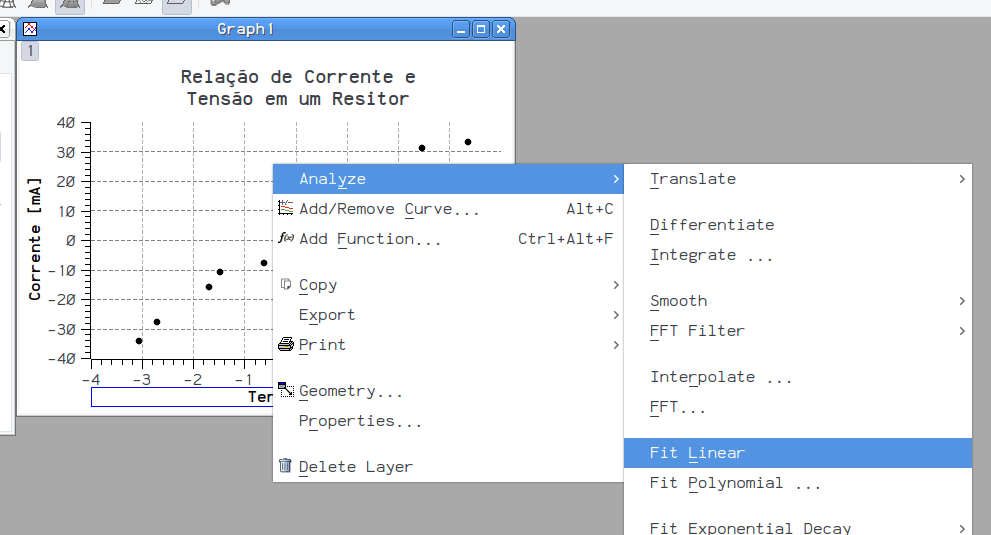
\includegraphics[width=0.7\textwidth]{regres/1regpath.png}

        \caption{Aplicando a regressão linear nos gráfico de exemplo (figura \ref{fig:reta:gridlinscat})}
        \label{fig:regres:path}
    \end{figure}


\subsection{Valores dos Coeficientes}

    Os valores dos coeficientes encontrados com a regressão aparecem em um \textit{log} sobre a janela da tabela e do gráfico dentro do \software.

    \begin{figure}[htbp]
        \centering
        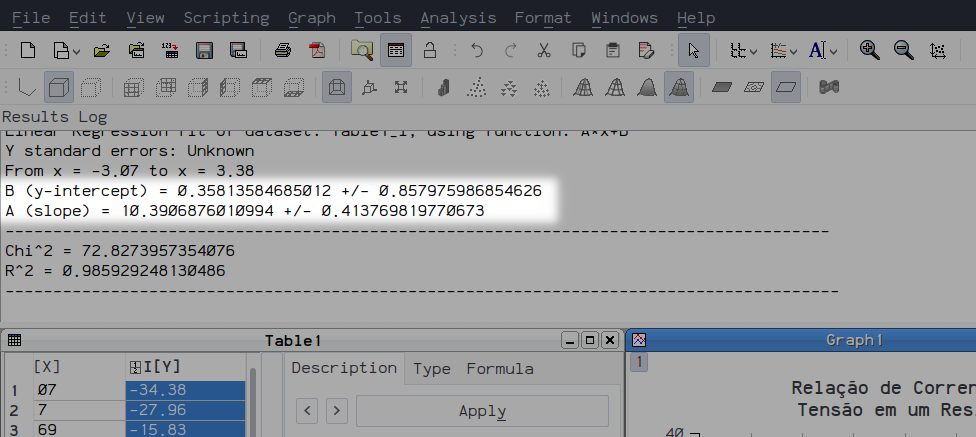
\includegraphics[width=0.6\textwidth]{regres/2coefs.png}

        \caption{Resultado com os coeficientes encontrados para a regressão}
        \label{fig:regres:coefs}
    \end{figure}


\subsection{Resultado}

    \begin{figure}[H]
        \centering
        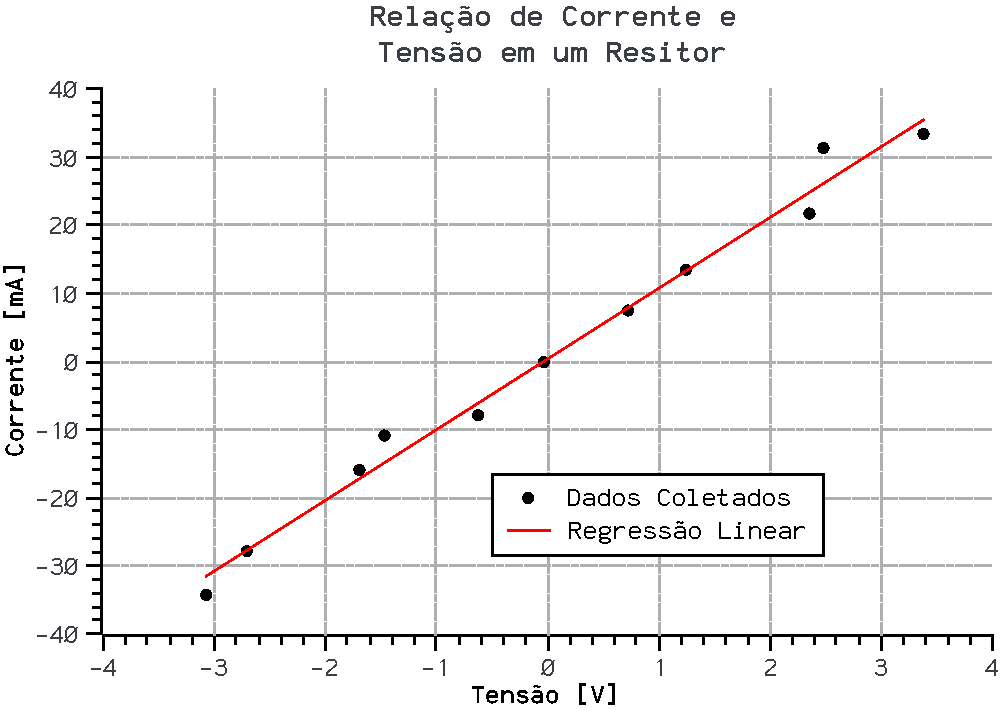
\includegraphics[width=0.6\textwidth]{regres/resultado.pdf}

        \caption{Exemplo de regressão linear}
        \label{fig:regres:final}
    \end{figure}
